\documentclass[11pt, a4paper]{article}

% ── Encoding & fonts ──────────────────────────────────────────────────────────
\usepackage[utf8]{inputenc}
\usepackage[T1]{fontenc}
\usepackage{lmodern}

% ── Page geometry ─────────────────────────────────────────────────────────────
\usepackage[margin=1in]{geometry}

% ── Hyperlinks & auto-updating TOC ────────────────────────────────────────────
\usepackage[hidelinks]{hyperref}   % hidelinks = no ugly red boxes

% ── Math ──────────────────────────────────────────────────────────────────────
\usepackage{amsmath, amssymb, amsthm}

% ── Misc useful packages ──────────────────────────────────────────────────────
\usepackage{tabularx}              % equal-width wrapping columns
\usepackage{enumitem}              % tighter lists
\usepackage{parskip}               % space between paragraphs instead of indent
\usepackage{caption}

% ── Theorem-like environments (optional, delete if not needed) ─────────────────
\newtheorem{theorem}{Theorem}[section]
\newtheorem{lemma}[theorem]{Lemma}
\theoremstyle{definition}
\newtheorem{definition}[theorem]{Definition}
\newtheorem{example}[theorem]{Example}
\theoremstyle{remark}
\newtheorem*{remark}{Remark}

%tikz
\usepackage{tikz}
\usetikzlibrary{arrows.meta, positioning, fit, backgrounds, patterns}


% Code blocks
\usepackage{listings}
\usepackage{xcolor}

\lstset{
    basicstyle=\ttfamily\small,
    keywordstyle=\color{blue},
    commentstyle=\color{gray},
    stringstyle=\color{teal},
    numbers=left,
    numberstyle=\tiny\color{gray},
    numbersep=8pt,
    breaklines=true,
    frame=single,
    captionpos=b,
}

\lstnewenvironment{cppcode}[1][]{\lstset{language=C++, #1}}{}
\lstnewenvironment{pycode}[1][]{\lstset{language=Python, #1}}{}
\lstnewenvironment{ccode}[1][]{\lstset{language=C, #1}}{}
\lstnewenvironment{bashcode}[1][]{\lstset{language=bash, #1}}{}
\newcommand{\code}[1]{\lstinline|#1|}

% ── Chapters & appendices in any order ────────────────────────────────────────
% \chap{<n>}{Title}, \app{<n>}{Title} (1=A, 2=B, ...)
\newcommand{\chap}[2]{%
  \renewcommand{\thesection}{\arabic{section}}%
  \renewcommand{\theHsection}{chap.\arabic{section}}%
  \setcounter{section}{#1}\addtocounter{section}{-1}%
  \section{#2}}
\newcommand{\app}[2]{%
  \renewcommand{\thesection}{\Alph{section}}%
  \renewcommand{\theHsection}{app.\Alph{section}}%
  \setcounter{section}{#1}\addtocounter{section}{-1}%
  \section{#2}}


% ── Document metadata ─────────────────────────────────────────────────────────
\title{Operating Systems: Three Easy Pieces}
\author{Andrea and Remzi Arpaci-Dusseau}
\date{\today}

% ──────────────────────────────────────────────────────────────────────────────
\begin{document}

\maketitle
\tableofcontents          % auto-updates on every compile (needs 2 passes)
Order: 13, 15, 16, 17, 18, 19, 20, 21, 22, 23, 26, 27, 28, 29, 30, 31, 32, 33, 7, 8, 10, 9, 14, 36, 39, 40, 42, 37, 44, 45, 38, 41, 43, 47, 48, 49, 50, 51
\newpage
\subsection{Introduction to Operating Systems}
\begin{itemize}
  \item Crux of the problem: How does the operating system virtualize resources?
  \begin{itemize}
    \item What mechanisms and policies are implemented by the OS to attain virtualization?
    \item How does the OS do this efficiently?
    \item What hardware support is needed?
  \end{itemize}
  \begin{definition}[Virtualization]
    The process in which the operating system takes a physical resource and abstracts it into an easier-to-use virtual form.
  \end{definition}
  \begin{definition}[System call]
    An interface or API exposed to the user to tell the OS what to do. A typical OS will export on the order of hundreds of system calls (syscall) 
  \end{definition}
  \item The OS is also responsible for managing resources, each of the CPU, memory, and disk.
\end{itemize}
\begin{ccode}
int main(int argc, char *argv[]) {
  if (argc != 2) { 
    fprintf(stderr, "usage: cpu <string>\n");
    exit(1);
  }
  char *str = argv[1];
  for (;;) {
    Spin(1);
    printf("%s\n", str);
  }
  return 0;
}
\end{ccode}
\begin{itemize}
  \item The above code will simply just print the string that the user passed, forever. 
  \item Interestingly though, even on a single core system we can run this program in parallel and all programs will run at the same time.
  \item The OS will virtualize each physical CPU into a seemingly infinite number of virtual CPUs, giving the illusion as if there are more than one.
  \item The OS policies defines the behaviour of the OS, including things like what programs get priority and what actions are permitted. 
  \item A similar idea is applied with memory: memory is just an array of bytes. 
  \item To read/write to memory, one needs to supply the address of whatever you want to access. 
  \item Consider a program that allocates some memory, prints the address of the memory \texttt{p} and writes the number 0 into the first slot of the allocated memory. Finally it loops and increments the value stored at the address held in \texttt{p}. 
  \item Similar to the example from before, if we run multiple instances of this program, then each instance will have allocated memory at the exact same address and each are updating the value at that address independently. 
  \item This is an example of the OS virtualizing memory; each process has it's own private virtual address space. 
  \item It is the OS's responsibility to map the virtual memory of each process to some portion of physical memory.
  \item Persistence: The OS is also responsible for ensuring that data that is stored in a volatile manner (such as DRAM) is not lost when power is lost or the system crashes. This is done through the usage of input/output, or I/O devices.
  \item Common IO devices in modern computers are hard drives or SSDs.
  \item Unlike the abstractions the OS performs on the physical CPU(s) and memory, there is no virtualization performed for each application. 
  \item It is assumed that the user wants to share the contents of a file; one application may be used to create and edit a file and another to compile. 
  \item The software that is responsible for managing and storing files on the disk is called the file system.
\end{itemize}
\newpage
\chap{4}{The Abstraction: The Process}
\begin{itemize}
  \item The crux of the problem: How to provide the illusion of many CPUs? In a system where there are only a few physical CPUs available, how can the OS provide the illusion of a nearly-endless supply of CPUs?
  \item The basic idea is simple: On a given CPU, the OS wil run one process, then stop it to run another process, and so on. This is known as \textbf{Time sharing}.
  \item Using this the OS can provide the illusion that one CPU is running multiple processes, at the cost of slower performance the more processes need to be shared on one CPU.
  \item Mechanisms: low-level methods or protocols that implement functionality.
  \item Policies: higher-level algorithms that are responsible for making some kind of decision within an OS. 
  \item A process at a given time can affect the memory that is reserved for it (its address space), as well as registers. 
  \item Special registers include the Program Counter/Instruction pointer (PC/IP), which tells what the next instruction to be executed is and a stack pointer is used to manage the stack for function parameters, local variables and return values. 
  \item Programs may also affect persistent storage devices as well. 
  \item The OS must expose the following APIs for processes:
  \begin{enumerate}
    \item Create: An OS must be able to create a new process. 
    \item Destroy: An OS must be able to destroy an existing process. 
    \item Wait: It is sometimes useful to wait for a specific process to stop 
    \item Misc. control: Some way to temporarily halt and resume a process 
    \item Status: Read-only APIs that give status info or some other pieces of metadata on a process.
  \end{enumerate}
\end{itemize}
\subsection{Process Creation}
\begin{itemize}
  \item The first thing the OS does is load the program code and any static data into memory (the address space of the process)
  \item This is done lazily; the OS will only fetch pieces of code or data that is necessary (opposed to eagerly). This is done to further support paging and swapping. 
  \item The OS then allocates memory on the program's stack as well as the heap. 
  \item It will then perform any remaining initialization tasks, such as those pertaining to IO. The OS then transfers control of the CPU to the newly-created process. 
\end{itemize}
\subsection{Process States}
In a simplified view, a process can be in one of three states:
\begin{enumerate}
  \item Running: The process is currently being executed. 
  \item Ready: A process is ready to run but is not currently being executed for some reason from the OS. 
  \item Blocked: A process has performed some operation in which it needs to wait for in order to proceed. An example is an IO request, in which the process needs to wait for the data to be fetched and is thus blocked; in the meantime some other process is free to use the processor.
\end{enumerate}


\begin{center}
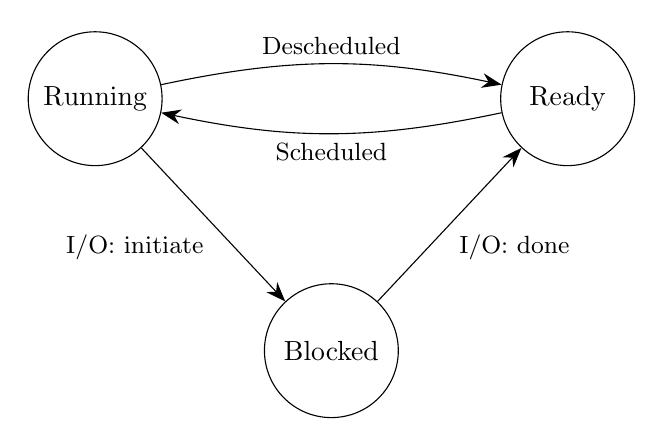
\begin{tikzpicture}[
    state/.style = {circle, draw, minimum size=17mm, align=center},
    every edge/.style = {draw, -{Stealth[length=2.5mm]}},
    lbl/.style = {font=\small}
  ]
  % nodes at explicit coordinates (in cm) so Blocked sits centred below the pair
  \node[state] (running) at (0, 0)    {Running};
  \node[state] (ready)   at (6, 0)    {Ready};
  \node[state] (blocked) at (3, -3.2) {Blocked};

  % edges: label side is chosen by auto / auto+swap so nothing overlaps a line
  \path (running) edge [bend left=12] node[lbl, above]      {Descheduled}   (ready);
  \path (ready)   edge [bend left=12] node[lbl, below]      {Scheduled}     (running);
  \path (running) edge                node[lbl, auto, swap] {I/O: initiate} (blocked);
  \path (blocked) edge                node[lbl, auto, swap] {I/O: done}     (ready);
\end{tikzpicture}
\end{center}
Below is an example for how two processes may transition through some of the states as shown in the diagram above:
\begin{center}
\begin{tabular}{c c c c}
\textbf{Time} & $\textbf{Process}_0$ & $\textbf{Process}_1$ & \textbf{Notes} \\
\hline
1  & Running & Ready   &                                    \\
2  & Running & Ready   &                                    \\
3  & Running & Ready   & $\text{Process}_0$ initiates I/O   \\
4  & Blocked & Running & $\text{Process}_0$ is blocked,     \\
5  & Blocked & Running & so $\text{Process}_1$ runs         \\
6  & Blocked & Running &                                    \\
7  & Ready   & Running & I/O done                           \\
8  & Ready   & Running & $\text{Process}_1$ now done        \\
9  & Running & --      &                                    \\
10 & Running & --      & $\text{Process}_0$ now done        \\
\end{tabular}
\end{center}
\subsection{Data Structures}
\begin{itemize}
  \item The process list will contain all processes that are ready and some extra information for what processes are currently running. 
  \item The OS must also keep track of blocked processes. 
  \item The register context will hold the contents of the registers of a stopped process. The registers of a stopped process are written to memory, and are restored when the process resumes. 
\end{itemize}
Below is an example of some data structures used in the xv6 kernel:
\newpage
\begin{ccode}
// the registers will save and restore to stop and restart a process 
struct context {
  int eip;
  int esp;
  int ebx;
  int ecx;
  int edx;
  int esi;
  int edi;
  int edp;
};

// the possible states a process can be in:
enum proc_state { UNUSED, EMBRYO, SLEEPING, RUNNABLE, RUNNING, ZOMBIE };

// the information xv6 tracks about each process 
struct proc {
  char *mem; //start of process memory
  uint sz;
  char *kstack; // bottom of kernel stack for this process
  enum proc_state state;
  int pid;
  struct proc *parent;
  void *chan; // !zero -> sleeping on chan 
  int killed; // !zero -> killed 
  struct file *ofile[NOFILE]; // open files 
  struct inode *cwd; 
  struct context context;
  struct trapframe *tf;
}
\end{ccode}
As seen above there are more states that a process can be in than the three listed; 
\begin{itemize}
  \item An initial state for when it is being created 
  \item A final state where it has exited but has not yet been cleaned up (zombie)
\end{itemize}
\newpage
\chap{5}{Interlude: Process API}
\subsection{The \texttt{fork()} System Call}
See \texttt{p1.c} for an example.
\begin{itemize}
  \item Once the proces reaches the \texttt{fork()} syscall, the OS will create a (nearly) identical copy of the calling process, just in its own address space
  \item From the perspective of the OS, there are two copies of \texttt{p1.c} running, each about to return from \texttt{fork()}. 
  \item The child does not start at \texttt{main()}, but rather the site in which \texttt{fork()} was invoked.
  \item For the parent, \texttt{fork()} will return the PID of the child, and for the child it returns 0.
  \item The output is also not deterministic: either the child or parent may print first. This is determined by the CPU scheduler. 
\end{itemize}
\subsection{The \texttt{wait()} System Call}
See \texttt{p2.c} for an example.
\begin{itemize}
  \item In this example the parent invokes the \texttt{wait()} syscall, which blocks it until the child finishes executing. 
  \item This will ensure that the program is now deterministic, as the child will always print first. 
\end{itemize}
\subsection{The \texttt{exec()} System Call}
See \texttt{p3.c} for an example.
\begin{itemize}
  \item On success, \texttt{exec()} doesnt return
  \item It will take the current process and replaces it with a different executable and starts at \texttt{main()}.
\end{itemize}
\subsection{Motivating the API}
\begin{itemize}
  \item The seperation between \texttt{fork()} and \texttt{exec()} allows the shell to run code after the \texttt{fork()} but before the \texttt{exec()}.
  \item This can alter the environment of the program that is to be executed.
  \item The shell shows a prompt and waits for the user to type a command.
  \item It then forks a new child process, calls exec to run the program, and waits for the command to finish, in which it prompts the user again.
  \item The seperation between the fork and exec allows the shell to implement some useful behaviour, including:
\end{itemize}
\begin{bashcode}
prompt> wc p3.c > newfile.txt
\end{bashcode}
\begin{itemize}
  \item The > redirects the output of \texttt{wc p3.c} into \texttt{newfile.txt}. This is done by first forking a new child process and then opening \texttt{newfile.txt} before executing \texttt{wc p3.c}.
  \item This redirects the output from stdout to \texttt{newfile.txt}. See \texttt{p4.c} for an example.
  \item \texttt{close()} takes a file descriptor as a parameter, and deallocates it (for whichever process called it). Note that it does not stop/terminate any processes or free PIDs.
  \item The stdout fd is always 1 (defined via \texttt{STDOUT\_FILENO} and is now free), and \texttt{open()} will always return the lowest fd, which is now set to \texttt{p4.output}.
  \item \texttt{wc p4.c} then writes to \texttt{p4.output} instead of stdout.
\end{itemize}
\begin{center}
For the child process:
\begin{tabular}{c c c c c}
\hline
& fd 0 & fd 1 & fd 2\\
\hline
after \texttt{fork()} & tty & stdout & tty & (copied from parent) \\
after \texttt{close(1)} & tty & (free) & tty & \\
after \texttt{open(...)} & tty & \texttt{p4.output} & tty & open returns lowest fd = 1 \\
\hline
\end{tabular}
\end{center}
\begin{itemize}
  \item A similar implementation is done for \texttt{pipe()}, which lets you connect the output a process to the kernel pipe (or a queue), which connects to the input of another process. For example,
\end{itemize}
\begin{bashcode}
prompt> grep -o foo file | wc -l
\end{bashcode}
\begin{itemize}
  \item Will get the number of times foo appears in file and pipe it to wc.
\end{itemize}
\subsection{Process Control and Users}
\begin{itemize}
  \item \texttt{kill()} is used to send signals to a process, including directives to pause, die and other things. 
  \item On most shells, keystrokes can also send signals (ctrl-c sends SIGINT, graceful termination and ctrl-z sends SIGSTP, which pauses a program and can be resumed with something like \texttt{fg}.)
  \item A process should also implement the \texttt{signal()} syscall to catch different signals; for example, to cleanup resources when a SIGINT is issued.
  \item Modern systems require a strong notion of a "user" to ensure that different people have various levels of access to system resources and signals.
\end{itemize}
  \chap{6}{Mechanism: Limited Direct Execution}
How to efficiently virtualize the CPU with control: The OS must virtualize the CPU in an efficient manner while retaining control over the system. Both hardware and OS support is required. 
\subsection{Basic Technique: Limited Direct Execution}
\begin{itemize}
  \item A technique used by operating systems to run programs on the CPU while keeping control of system security and resources.
  \item "Direct execution" referes to the fact that programs run on the CPU 
\end{itemize}
\begin{center}
\begin{tabular}{c c}
\textbf{OS} & \textbf{Program} \\
\hline
Create an entry for process list & \\
Allocate memory for program & \\ 
Load program into memory & \\ 
Setup stack with argc and argv & \\ 
Clear registers & \\ 
Execute main() & \\
& Run main() \\
& Execute return from main() \\ 
Free memory of process & \\ 
Remove from process list & \\
\end{tabular}
\captionof{table}{Direct execution protol, no limits}
\end{center}
\begin{itemize}
  \item Issues: How do we restrict operations for specific programs? How do we implement time sharing to virtualize the CPU?
\end{itemize}
\subsection{Problem \#1: Restricted Operations}
How to perform restricted operations: A process must be able to perform I/O and some other (possibly) restricted operations, but wihtout giving the process full access over the system. How does the OS implement this while still executing as fast as possible?
\begin{definition}[User mode]
User mode is a restricted operating state. Code ran in user mode does not have access to certain operations, such as issuing I/O requests. Performing a restricted operation in user mode will cause the processor to raise an exception and the OS to kill the proces.
\end{definition}
\begin{definition}[Kernel mode]
The operating state in which the operating system (or kernel) runs in. There are no hardware-enforced restrictions in this mode. 
\end{definition}
\begin{itemize}
  \item System calls allow the kernel to expose pieces of kernel functionality to user programs, such as accessing file systems, creating and destroying processes, communicating with other processes and allocating memory.
  \item System calls are executed via trap instructions, which is a jump + elevation into kernel mode.
  \item When finished, the OS issues a return-from-trap instruction, which returns back to the user program and reduces priviledges to user mode.
  \item The kernel controls what code executes during a trap with a trap table (set on boot).
\end{itemize}
\begin{center}
\small
\begin{tabular}{c c c}
\textbf{OS @ boot (kernel mode)} & \textbf{Hardware} & \\
\hline 
\textbf{Initialize trap table} & & \\
& remember address of syscall handler & \\ 
\\ 
\textbf{OS @ run (kernel mode)} & \textbf{Hardware} & \textbf{Program (user mode)} \\ 
\hline
Create entry for process list & & \\
Allocate memory for program & & \\ 
Load program into memory & & \\ 
Setup user stack with argv & & \\ 
Fill kernel stack with reg/PC & &\\
\textbf{return-from-trap} & & \\
& restore regs(from kernel stack) & \\ 
& move to user mode & \\ 
& jump to main & \\ 
& & Run main() \\ 
& & /*executing..*/ \\ 
& & Call syscall \\ 
& & \textbf{trap} into OS \\ 
& save regs (to kernel stack) & \\ 
& move to kernel mode & \\ 
& jump to trap handler (from trap table) & \\ 
Handle trap & & \\ 
Do work for syscall & & \\ 
\textbf{return-from-trap} & & \\ 
& restore regs(from kernel stack) & \\ 
& move to user mode & \\ 
& jump to PC & \\
& & /*keep executing...*/ \\ 
& & return from main \\ 
& & \textbf{trap} invoked by \texttt{exit()} \\ 
Free memory of process & & \\ 
Remove from process list & &  
\end{tabular}
\captionof{table}{Limited Direct Execution Protocol}
\end{center}
\begin{itemize}
  \item The trap table contains various exceptions and one entry for syscalls (eg 0x80 on x86).
  \item When a syscall is invoked, a system-call number is assigned to each unique syscall. This tells the trap handler which syscall to invoke.
  \item User trap instruction -> hardware trap table -> syscall trap handler -> syscall table (seperate from trap table) -> do stuff
\end{itemize}
\subsection{Problem \#2: Switching Between Processes} 
Assuming a single core system: If a process is running on the CPU, then the OS is not running; how does it do anything?\\
Specifically, How can the operating system regain control of the CPU so that it can switch between processes?
\subsubsection{Cooperative approach: Wait for syscalls}
\begin{itemize}
  \item Most early operating systems
  \item A cooperative approach means that the OS will assume that long-running processes will periodically give up the CPU so that the OS can do some other stuff.
  \item This works as most processes frequenetly issue syscalls to the OS. 
  \item Cooperative operating systems also generally come with a yield syscall which transfers control to the OS so it can do stuff.
  \item Illegal operations (like dividing by 0, accessing restricted memory) will also generate traps for the OS so that it has control.
  \item However, this raises the question: How can the OS gain control of the CPU even if processes are not being cooperative?
\end{itemize}
\subsection{Non-cooperative approach}
\begin{itemize}
  \item Timer interrupt: An internal timer will make the hardware periodically issue interrupts to a process every few miliseconds; this will temporarily halt the process and give the OS control through a trap (via an interrupt handler).
  \item The hardware also has some responsibility during an interrupt: it needs to save enough of the state of the program just before the interrupt so that after the subsequent return-from-trap instruction the program can run correctly.
\end{itemize}
\subsubsection{Saving and Restoring Context}
\begin{itemize}
  \item The scheduler may decide to switch to a different process during an interrupt. 
  \item If this happens, the OS runs a context switch, which saves GPRs, the PC, and the kernel stack pointer for the current process and restores them for the process to be executed.
\end{itemize}
\begin{center}
\small
\begin{tabular}{c c c}
\textbf{OS @ boot (kernel mode)} & \textbf{Hardware} & \\
\hline 
\textbf{initialize trap table} & &  \\ 
& Remember address of syscall handler & \\ 
& and timer handler & \\
\textbf{start interrupt timer} & & \\
& start timer & \\
& interrupt CPU in X ms & \\
\\
\textbf{OS @ run (kernel mode)} & \textbf{Hardware} & \textbf{Program(user mode)} \\
\hline 
& & Process A \\
& & /* after X ms... */ \\ 
& \textbf{timer interrupt} & \\ 
& regs(A)->kernel stack(A) & \\ 
& move to kernel mode & \\ 
& jump to trap handler & \\ 
Handle the trap & & \\ 
Context switch: & & \\ 
  regs(A)->proc\_t(A) & & \\
  regs(B)<-proc\_t(B) & & \\
  switch to kernel stack(B) & & \\
\textbf{return from trap to B} & & \\
& regs(B)<-kernel stack(B) & \\ 
& move to user mode & \\
& jump to B's PC & \\
& & Process B \\
\end{tabular}
\captionof{table}{Limited Direct Execution Protocol (Timer Interrupt)}
\end{center}
\chap{13}{The Abstraction: Address Spaces}
\subsection{Early Systems}
Early OS designs would not abstract away physical address space (1 to 1 mapping).
\subsection{Multiprogramming and Time Sharing}
\begin{itemize}
  \item Multiprogramming: When multiple processes are ready to run at a given time, and the OS is responsible for deciding when to switch between them, for example during an IO request.
  \item This helped increase the effective utilization of the CPUa. 
  \item Time sharing: When the OS allows multiple users or tasks to share the same CPU by switching between them quicky.
  \item This was initially implemented my letting one process run for a short time (giving it full access to all memory), saving its state to some kind of disk, load the other process's state, and run it. 
  \item The limitation with this implementation is that it is extremely slow; while saving and restoring register-level information is fast, writing memory to disk is very slow.
\end{itemize}
\subsection{The Address Space}
The address space is an abstraction of physical memory which contains the memory state of the running program. 
\begin{itemize}
  \item This contains the program code, the heap, and the stack.
\end{itemize}
\begin{center}
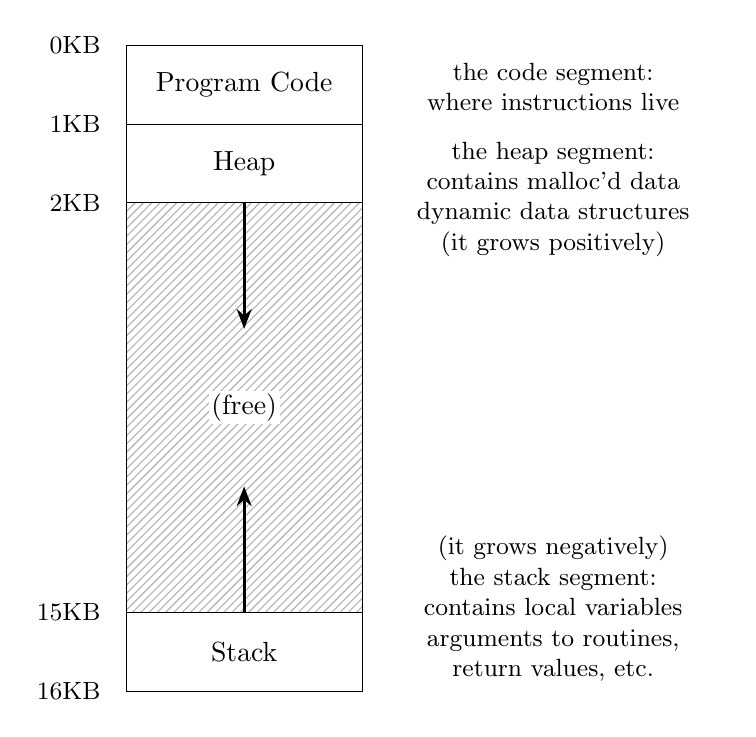
\begin{tikzpicture}[
    seg/.style    = {draw, minimum width=3cm, align=center},
    kb/.style     = {font=\small, anchor=east},
    note/.style   = {font=\small, align=center, text width=4.2cm},
    growth/.style = {-{Stealth[length=2.5mm]}, very thick}
  ]
  % segment boundaries (not to scale: free space is compressed)
  \def\w{3}
  \fill[pattern=north east lines, pattern color=gray!60] (0,-2) rectangle (\w,-7.2);
  \draw (0,0) rectangle (\w,-1) node[midway] {Program Code};
  \draw (0,-1) rectangle (\w,-2) node[midway] {Heap};
  \draw (0,-2) rectangle (\w,-7.2);
  \draw (0,-7.2) rectangle (\w,-8.2) node[midway] {Stack};
  \node[fill=white, inner sep=1pt] at (\w/2,-4.6) {(free)};

  % growth arrows
  \draw[growth] (\w/2,-2)   -- (\w/2,-3.6);
  \draw[growth] (\w/2,-7.2) -- (\w/2,-5.6);

  % addresses
  \node[kb] at (-0.2, 0)    {0KB};
  \node[kb] at (-0.2,-1)    {1KB};
  \node[kb] at (-0.2,-2)    {2KB};
  \node[kb] at (-0.2,-7.2)  {15KB};
  \node[kb] at (-0.2,-8.2)  {16KB};

  % annotations
  \node[note, anchor=north west] at (\w+0.2,-0.1) {the code segment:\\ where instructions live};
  \node[note, anchor=north west] at (\w+0.2,-1.1) {the heap segment:\\ contains malloc'd data\\ dynamic data structures\\ (it grows positively)};
  \node[note, anchor=south west] at (\w+0.2,-8.2) {(it grows negatively)\\ the stack segment:\\ contains local variables\\ arguments to routines,\\ return values, etc.};
\end{tikzpicture}
\captionof{figure}{An Example Address Space}
\end{center}
See \texttt{va.c} for an example of this.
\begin{itemize}
  \item Note that this is an abstraction from physical memory; the program isnt really loaded in memory at physical address 0 to 16KB.
  \item This abstracted address is called the virtual address, and the process in which the OS performs this abstraction is virtualizing memory. 
\end{itemize}
\subsection{Goals}
\begin{enumerate}
  \item Transparency: The OS should implement virtual memory in a way that is invisible to the running program; i.e. the running program should not be aware that the memory it is accessing is a virtual address.
  \item Efficiency: The OS should make virtualization as fast and as space-efficient as possible. This often requires hardware support (eg translation lookaside buffers)
  \item Protection: The OS must ensure that that one process cannot access or affect in any way the memory contents of any other processes (that are outside of its address space).
\end{enumerate}
\chap{14}{Interlude: Memory API}
In Unix/C programs, understanding how to allocate and manage memory is critical in building robust and reliable software. What interfaces are commonly used? What mistakes should be avoided?
\subsection{Types of Memory}
\begin{itemize}
  \item Stack memory is implicitly managed by the compiler (also known as automatic memory)
  \item When the variable goes out of its current scope it gets deallocated; thus heap memory is used for long lasting memory
\end{itemize}
\subsection{The \texttt{malloc()} Call}
\begin{itemize}
  \item Allocates memory on the heap, and returns either a pointer to the memory or NULL on fail. 
\end{itemize}
\begin{ccode}
void *malloc( size_t size ); // defined in header <stdlib.h>

// the return of malloc should be cast to the type of the underlying data.
double *d = (double *) malloc(sizeof(double));
\end{ccode}
\subsection{The \texttt{free()} Call}
This frees memory that has been previously allocated on the heap. 
\begin{ccode}
void free( void *ptr ); // defined in header <stdlib.h>
\end{ccode}
\begin{itemize}
  \item Note that it is UB if \texttt{ptr} does not equal a value returned by one of malloc's variants. \\
  \item Using \texttt{ptr} after it has been freed is undefined (use-after-free). \\
  \item It is unddefined if the memory area referred to by \texttt{ptr} has already been deallocated (double-free).
  \item If your proaram is short-lived, it may not be necessary (albeit bad practice) to free memory, as the address space of a program gets wiped on return.
\end{itemize}
\subsection{Underlying OS Support}
\begin{itemize}
  \item Note that \texttt{malloc} and \texttt{free} are not syscalls; instead they are implemented by third party libraries (such as libc) which act as thin wrappers around syscalls.
  \item One syscall is \texttt{brk}, which changes the location of the end of the program's break or heap.
  \item \texttt{mmap} is another syscall that requests an anonymous memory region within a program, which is not associated with that particular program and can thus be shared with other programs/processes (memory mapped via \texttt{mmap} is in swap space} which act as thin wrappers around syscalls.
  \item One syscall is \texttt{brk}, which changes the location of the end of the program's break or heap.
  \item \texttt{mmap} is another syscall that requests an anonymous memory region within a program, which is not associated with that particular program and can thus be shared with other programs/processes (memory mapped via \texttt{mmap} is in swap space}).
\end{itemize}
\chap{15}{Mechanism: Address Translation}
How can we build an efficient virtualization of memory?
\begin{itemize}
  \item The OS needs to have both efficiency and control over the program when virtualizing memory.
  \item Make use of hardware support whenever possible (registers, TLB, page-tables, etc.)
  \item Ensure no application is able to access any memory but its own
  \item \textit{Hardware-based address translation}: Also known as just address translation for short - On any memory access, the hardware transforms the virtual address to the physical location of the data requested.
  \item It is the hardware's responsibility to translate virtual addresses to the physical locations and enforce protection (bounds and permission checks).
  \item The OS is responsible for keeping track of occupied and free physical locations, setup, and exception handling.
  \item This becomes more complicated when you factor in the fact that different program's address spaces may have the same virtual address but map to different physical locations which the OS must keep track of.
  \item Interposition: Placing a layer in between the software and an interface to add some extra functionality. Interposition (should) be invisible to the caller. 
  \item In the context of virtualizing memory, the hardware interposes every memory access by translating the virtual address to a physical location.
\end{itemize}
\subsection{Assumptions}
For now, assume:
\begin{itemize}
  \item User address space must be contiguous in physical memory. 
  \item User address space is smaller than the size of physical memory. 
  \item Each address space is exactly the same size
\end{itemize}
\subsection{Example}
Consider:
\begin{ccode}
void func() {
  int x = 3000;
  x = 3 + 3; // line of code we are interested in
  /* ... */
}
\end{ccode}
With no optimizations (x86):
\begin{bashcode}
; ... 
movl -8(%rbp), %eax 
addl $3, %eax 
movl %eax, -8(%rbp)
; ...
\end{bashcode}
\begin{itemize}
  \item x is a local variable at address \texttt{\%rbp - 8}, and gets moved into register eax. 
  \item Add the constant 3 
  \item Move x out of eax back into its stack address
  \item From the program's perspective, its address space starts at 0 to some number (say, 16KB).
  \item The OS needs to place the process somewhere else, not necessarily starting at address 0. How?
\end{itemize}
\subsection{Dynamic Relocation}
\begin{itemize}
  \item Also known as base and bounds, this is a hardware-based technique, where each CPU requires two hardware registers, the base and bounds (or limit) register.
  \item Each program is compiled as if it starts at address 0.
  \item When a process is loaded, the OS decides where in physical memory to place the program and sets the base register to this value. 
  \item Once the program starts running, it adds the base register value to get the physical address
\end{itemize}
\begin{align*}
\text{physical address} = \text{virtual address} + \text{base}
\end{align*}
\begin{itemize}
  \item Note that the interposition ensures that no "add base register" ever shows up in the instructions themselves (interposition is invisible)
  \item Address translation: transforming a virtual address into a physical address 
  \item Since the addressing happens at runtime (base register is set when the program is compiled and loaded), it is dynamic relocation.
  \item The bounds register is used to ensure that no accesses exceed the program's address space
  \item Bounds register stores the program size (virtual address of the largest allowed memory access, starting at 0); exception is raised before translation.
  \item The portion of the CPU that handles address translation is called the memory-management unit (MMU).
  \item Example: consider a process with an address space of 4KB that is loaded at physical address 16KB.
  \item Base register is set to 16KB, Bounds register is set to 4KB
\end{itemize}
\begin{center}
\begin{tabular}{c c c}
  \textbf{Virtual Address} && \textbf{Physical Address} \\
  \hline 
  0 & $\rightarrow$ & 16KB \\ 
  1KB & $\rightarrow$ & 17KB \\ 
  3000 & $\rightarrow$ & 19384 \\ 
  4400 & $\rightarrow$  & \textit{fault (out of bounds)} \\
\end{tabular}
\end{center}
\subsection{Hardware support: A summary} 
\begin{itemize}
  \item The hardware must have support for two different modes: kernel mode and user mode. 
  \item A single bit is usually used for this to indicate which mode the CPU is currently running in. 
  \item Hardware must also provide base nad bound registers, plus the MMU of the CPU.
\end{itemize}
\subsection{Operating System Issues}
Responsibilities of the OS include:
\begin{itemize}
  \item OS must find space in physical memory for a newly created process (under our assumptions, this should be trivial).
  \item The OS will search a \textbf{free list} which lists ranges of physical memory not currently in use to find where to place the process. 
  \item The OS must put the memory of a process back on the free list on exit. 
  \item Since each CPU only has one base-bounds register pair, it must save the contents of these registers when context switching into some per-process area such as the process structure or process control block.
  \item The OS must provide exception handlers; these handlers are configured at boot time. On most exceptions the OS will terminate the process that caused the exception.
\end{itemize}
\begin{center}
\begin{tabular}{c c c}
\textbf{OS @ boot} & \textbf{Hardware} & \textbf{No program yet} \\ 
\hline 
\textbf{initialize trap table} & & \\
& Remember addresses of... & \\
& syscall handler & \\ 
& timer handler & \\ 
& illegal mem-access handler & \\ 
& illegal instruction haldner & \\ 
\textbf{start interrupt timer} & &\\
& start timer; interrupt every X ms & \\ 
\textbf{initialize process table} & & \\
\textbf{initialize free list} & & \\
\end{tabular}
\end{center}
\end{document}
